%%
%% This is file `sample-manuscript.tex',
%% generated with the docstrip utility.
%%
%% The original source files were:
%%
%% samples.dtx  (with options: `manuscript')
%% 
%% IMPORTANT NOTICE:
%% 
%% For the copyright see the source file.
%% 
%% Any modified versions of this file must be renamed
%% with new filenames distinct from sample-manuscript.tex.
%% 
%% For distribution of the original source see the terms
%% for copying and modification in the file samples.dtx.
%% 
%% This generated file may be distributed as long as the
%% original source files, as listed above, are part of the
%% same distribution. (The sources need not necessarily be
%% in the same archive or directory.)
%%
%% The first command in your LaTeX source must be the \documentclass command.
\documentclass[manuscript,screen]{acmart}

\graphicspath{{Fig/}}

%%
%% \BibTeX command to typeset BibTeX logo in the docs
\AtBeginDocument{%
  \providecommand\BibTeX{{%
    \normalfont B\kern-0.5em{\scshape i\kern-0.25em b}\kern-0.8em\TeX}}}

%% Rights management information.  This information is sent to you
%% when you complete the rights form.  These commands have SAMPLE
%% values in them; it is your responsibility as an author to replace
%% the commands and values with those provided to you when you
%% complete the rights form.
% \setcopyright{acmcopyright}
% \copyrightyear{2020}
% \acmYear{2020}
% \acmDOI{10.1145/1122445.1122456}


%% These commands are for a PROCEEDINGS abstract or paper.


% \acmConference[Woodstock '18]{Woodstock '18: ACM Symposium on Neural
%   Gaze Detection}{June 03--05, 2018}{Woodstock, NY}
% \acmBooktitle{Woodstock '18: ACM Symposium on Neural Gaze Detection,
%   June 03--05, 2018, Woodstock, NY}
% \acmPrice{15.00}
% \acmISBN{978-1-4503-XXXX-X/18/06}


%%
%% Submission ID.
%% Use this when submitting an article to a sponsored event. You'll
%% receive a unique submission ID from the organizers
%% of the event, and this ID should be used as the parameter to this command.
%%\acmSubmissionID{123-A56-BU3}

%%
%% The majority of ACM publications use numbered citations and
%% references.  The command \citestyle{authoryear} switches to the
%% "author year" style.
%%
%% If you are preparing content for an event
%% sponsored by ACM SIGGRAPH, you must use the "author year" style of
%% citations and references.
%% Uncommenting
%% the next command will enable that style.
%%\citestyle{acmauthoryear}

%%
%% end of the preamble, start of the body of the document source.
\begin{document}

%%
%% The "title" command has an optional parameter,
%% allowing the author to define a "short title" to be used in page headers.
\title{SUSI GENE: a portable robot as venting, recording  and sharing tool for improving mental health condition}

%%
%% The "author" command and its associated commands are used to define
%% the authors and their affiliations.
%% Of note is the shared affiliation of the first two authors, and the
%% "authornote" and "authornotemark" commands
%% used to denote shared contribution to the research.



% \author{Tingliang Zhang}
% \authornote{Both authors contributed equally to this research.}
% \email{ztl20@mails.tsinghua.edu.cn}
% \orcid{0000-0002-0164-4700}
% \author{Hua Tong}
% \authornotemark[1]
% \email{Constanzatong@gmail.com}
% \affiliation{%
%   \institution{Tsinghua University}
%   \streetaddress{Qinghuayuan, Haidian District}
%   \city{Beijing}
%   \country{China}
%   \postcode{100084}
% }

% \author{Yitong Wang}
% \authornote{Both authors contributed equally to this research.}
% \email{3bastet@163.com}
% \author{Meiqi Tu}
% \authornotemark[2]
% \email{@gmail.com}
% \affiliation{%
%   \institution{Tsinghua University}
%   \streetaddress{Qinghuayuan, Haidian District}
%   \city{Beijing}
%   \country{China}
%   \postcode{100084}
% }

% \author{Danni Liu}
% \affiliation{%
%   \institution{University of Washington}
%   \streetaddress{Qinghuayuan, Haidian District}
%   \city{Seattle}
%   \state{Washington}
%   \country{United States}
% }
% \email{dnliudanni@gmail.com}



% \author{Haipeng Mi}
% \affiliation{%
%   \institution{Tsinghua University}
%   \streetaddress{Qinghuayuan, Haidian District}
%   \city{Beijing}
%   \country{China}
%   \postcode{100084}
% }
% \email{mhp@mail.tsinghua.edu.cn}

%%
%% By default, the full list of authors will be used in the page
%% headers. Often, this list is too long, and will overlap
%% other information printed in the page headers. This command allows
%% the author to define a more concise list
%% of authors' names for this purpose.
\renewcommand{\shortauthors}{Zhang and Tong, et al.}

%%
%% The abstract is a short summary of the work to be presented in the
%% article.
\begin{abstract}

  Mental health condition is a major challenge throughout the world, yet mental health services in many countries are struggling to meet such needs. Studies have shown innovative intervention can have positive impacts on patients' mental health conditions. This paper presents SUSI GENE, an egg-shaped portable robot, designed for people with mood disorders, including major depressive disorder, bipolar disorder, etc. Through interactions, SUSI GENE attempts to help patients increase their self-awarenesses, vent their emotions, face their inner conflicts, and reappraise their problems in a less negative approach.

\end{abstract}

  % SUSI GENE is an egg-shaped interactive robot that designed for mental disordered people. It can be placed on the back of  a smart phone.SUSI is a safe, friendly and portable tool to prevent depression disorder and assist patients with mental disorders (such as depression disorder). It help people by increasing self-awareness, assisting treatment and seeking help. It encourages people who are experiencing emotional problems to expose and face their inner vulnerability in an appropriate way, so as to help them vent emotions and carry out cognitive reappraisal.

%%
%% The code below is generated by the tool at http://dl.acm.org/ccs.cfm.
%% Please copy and paste the code instead of the example below.
%%
\begin{CCSXML}
  <ccs2012>
     <concept>
         <concept_id>10003120.10003123.10010860.10010858</concept_id>
         <concept_desc>Human-centered computing~User interface design</concept_desc>
         <concept_significance>500</concept_significance>
         </concept>
     <concept>
         <concept_id>10003456.10010927.10003616</concept_id>
         <concept_desc>Social and professional topics~People with disabilities</concept_desc>
         <concept_significance>500</concept_significance>
         </concept>
     <concept>
         <concept_id>10010583.10010584.10010587</concept_id>
         <concept_desc>Hardware~PCB design and layout</concept_desc>
         <concept_significance>300</concept_significance>
         </concept>
     <concept>
         <concept_id>10003120.10003121.10003125.10010597</concept_id>
         <concept_desc>Human-centered computing~Sound-based input / output</concept_desc>
         <concept_significance>300</concept_significance>
         </concept>
     <concept>
         <concept_id>10010405.10010444.10010446</concept_id>
         <concept_desc>Applied computing~Consumer health</concept_desc>
         <concept_significance>500</concept_significance>
         </concept>
   </ccs2012>
\end{CCSXML}

\ccsdesc[500]{Human-centered computing~User interface design}
\ccsdesc[500]{Social and professional topics~People with disabilities}
\ccsdesc[300]{Hardware~PCB design and layout}
\ccsdesc[300]{Human-centered computing~Sound-based input / output}
\ccsdesc[500]{Applied computing~Consumer health}
%%
%% Keywords. The author(s) should pick words that accurately describe
%% the work being presented. Separate the keywords with commas.
\keywords{datasets, neural networks, gaze detection, text tagging}


%%
%% This command processes the author and affiliation and title
%% information and builds the first part of the formatted document.
\maketitle

\section{Introduction}

\subsection{What is susi gene}

SUSI GENE is an interactive emotion assistant.  It consists of a tangible egg-shaped robot along with an interface. The robot receives vocal inputs from a user; the mobile phone converts that radio to text for natural language processing; while the interface accordingly generates a virtual creature for the user as well as documents these data.

Past research indicated that people with mood disorders demonstrate overall satisfaction with the usage of mobile technology to increase their mental well-being.\cite{proudfoot2010community}
A large variety of products and research prototypes have made it possible for people to self-monitor their mental conditions, but most of these systems are designed as apps on mobile devices, and thus do not involves tangible interactions.

SUSI GENE also incorporates recording capabilities and requires some operations on mobile devices. However, it has several significant differences. We designed SUSI GENE as an egg-shaped portable robot aims to provide the user a more intuitive experience while sharing his or her stories and feelings. 

\subsection{How susi gene works}

For our current prototype, the user is expected to talk directly to the egg and hold the button that corresponding to his or her current emotion. There are eight emotions, each of them is corresponding to a button with a unique shape. After that, the user needs to place the egg on the back of a mobile device and, through the usage of Near-Field-Communication(NFC) technology, wait for the device pairs with the robot to receive and interpret the piece of audio and vibrates as a feedback signal. During that time, the radio is converted to text for natural language processing(NLP), the text would be split into several keywords. The selected keywords would be analyzed in reference to the HowNet and NTUSD sentiment lexicon, and the “emotion gene” is therefore finalized. After a brief vibration, a creature would hatch out and shown on the screen. The picture of the generated creature and the radio of his or her words will be saved for later usage. The user can not only review those past experiences but also share them to his or her friends, family members, or professional counsellors.

The interactive process imitates the natural hatching of the oviparity animals. Our design assumption is that the process of the young break through its shell is especially inspiring and may bring positive impact on the level of enjoyment.\cite{nezlek2008regulating}

FIGURE

It is often found that people noticed they were holding some negative emotions and at the same time, felt bad for this fact and therefore were more prone to negative emotions. We wish to convey the idea that all emotions can hatch out lovely creatures and thus guide the users away from making value judgment about different emotions.

We select eight emotions which are tranquil, contented, joyful, excited, fatigued, upset, anxious and angry as the identification bases, and inspired by Hanada,\cite{hanada2018correspondence}
we arrange them from two dimensions: pleasantness and arousal level. Based on previous studies in color psychology,\cite{valdez1994effects}
we assigned specific shapes and colors to each emotion to facilitate identification. The two emotions with similar arousal level, such as tranquil and fatigued, share a basic pattern but varies in colors and edges. The pattern demonstrate emotions that are considered relatively pleasureless have sharped edges and in darker colors, whereas the pattern presented other emotions have rounded edges and in brighter colors. 

These shapes and colors also become the bases for creature generation. The eight emotions respectively matches eight kinds of creatures. In general, the emotions relates to pleasure are either represented by plants or warm blood animals, and the emotions relates to displeasure are visualized as fungus and cold blood animals. In this prototype, the kinds of animals along with their basic appearances and backstories are pre-defined (some of the settings are illustrated below), but the additional information provided by the user is supposed to affect how the detailed components finalize. In our future versions, we expect to make the generated creature more unique and personalized by altering more elements of the creature.

\begin{itemize}
  \item Cacited: Cacited is a cat-like creature. Cacited’s ancestor lived in alpine region and that endows his exceptional speed and hunting skill. His eyes and ear would shine after a successful hunting.
  \item Repgry: Repgry has jagged fins on its cheeks and acicular scales on its body. It lives in desert area and lack of water makes its fins and scales change from soft to hard. Repgry has always been trying to stay closer to water since he worries other animals would avoid him because of his appearance.
  \item Anxect: Anxect is very small—about 4 millimeter long, and so is his heart. Thus, Anxect’s pulse may suddenly race, and he has to vibrate his wings quickly to reduce the symptoms. During that process, he might unexpectedly finish a long journey. 
  \item Upsafish: Upsafish is a type of mollusk living in the sea. He has two forms. In normal state, he looks like an octopus, and during cloudy days, he would grow into a whale tail  and shows some spots on his skins until the sun returns.
\end{itemize}


\section{Background}

Today, mood disorder, including depression, has became the worldwide leading cause of the Years Lived with Disability (YLDs). Many countries have started to pay increased attentions to people’s mental health conditions, and a number of plans aimed to make mental health services more accessible have emerged. However, most of these approaches, including one-to-one counseling, are mostly resource-intensive since each patient should be addressed individually.\cite{world2019special}

According to Monroe and Simons' model, the factors causing psychopathology can be basically concluded as diathesis (predisposition/vulnerability) and stress (triggers).\cite{monroe1991diathesis}
The model suggests all individual, no matter having what innate diathesis, has possibility to develop mood disorder under certain amount of stress, and proper react mechanism to the event of stress is the main solution to reduce that possibility. Considering the foreseeable shortage of mental health services, it is of crucial importance to find innovative interventions to help people with mood disorder in all stages, especially when they remain undiagnosed. Based on the interview of 11 subjects who suffer from mental disorder, we locate two situations that most likely cause and even continuously worsen a person’s mental health problem, which are:

\begin{enumerate}
  \item low-recognition of stress-caused emotion changes
  \item emotion-driven social isolating
\end{enumerate} 

Recent research and products provide solutions by replacing the communicatee from human beings to algorithms. However, there is little interactive solution focusing on changing these two mechanisms by guiding the individual to apply new actions to improve their overall mental qualities.

Therefore, we designed SUSI GENE: a robot with tangible interface to help users sharing their stress event and related emotion changes through a gamified process. Our design is based on cognitive-behavioral therapy(CBT), which asks patient to record the process of how their generate a certain emotion, and by doing this, helps patients deconstruct as well as change their previous beliefs toward a more positive mindset.

\section{Design}

Because the egg has a symbol of new life, it is used as a source of inspiration, implying that emotions can be broken.

And start the egg by touching the recording function to the user. The natural source of the vibration is the vibration of the shell. The translucent eggshell can use light as feedback during its use, and these slowly changing lights can soothe people's emotions.

The size is in line with ergonomics. It is designed to be a smooth and round surface that can be held in the palm of the hand to give people a relaxing experience. Palm toys have a long history. The rosary beads in Buddhist hands and small stones in Egyptian hands are all like this, which can stabilize emotions. In the same way, this egg has a similar function.

In the design of the icon, we choose eight kinds of emotions as the representative and energy drive to design two sets of positive and negative icons, and use different colors to represent them. In order to guide users to cherish and contain their own emotions, the emotional symbols with different images are designed to relax, full of expectations and gradually accept themselves in the process of waiting for their emotional animals to break their shells.

In the design of Metazoa, there are no unique fantasy animals designed by combining different animals. Because of the complexity of emotions, each animal will have other emotional characteristics, including but not limited to graphics and colors. This emotional animal of each user provides more possibilities and is a unique emotional animal for users.

\section{Hardware}

SUSI Gene is an egg-shaped portable robot, its dimensions are 62 mm in diameter and 80 mm in height. Its center of gravity is low, so it can stand on the back of the phone like a tumbler.

The SUSI Gene prototype is comprised of three main hardware components: the main PCB with an Arduino NANO BLE Sense and other necessary components on it, a battery, and a 3D printed shell.

\subsection{Main PCB design}

The main PCB integrates Arduino Nano 33 BLE Sense (with headers), a battery connector, 6 individually addressable Warm White RGBW version WS2812B with integrated drivers, a connector for vibration motor, and an I2C port for NFC chip communication.

The main PCB schematic is shown in Fig~\ref{PCBsch1} and its layout is shown in Fig~\ref{PCB1}.

\begin{figure}[h]
  \centering
  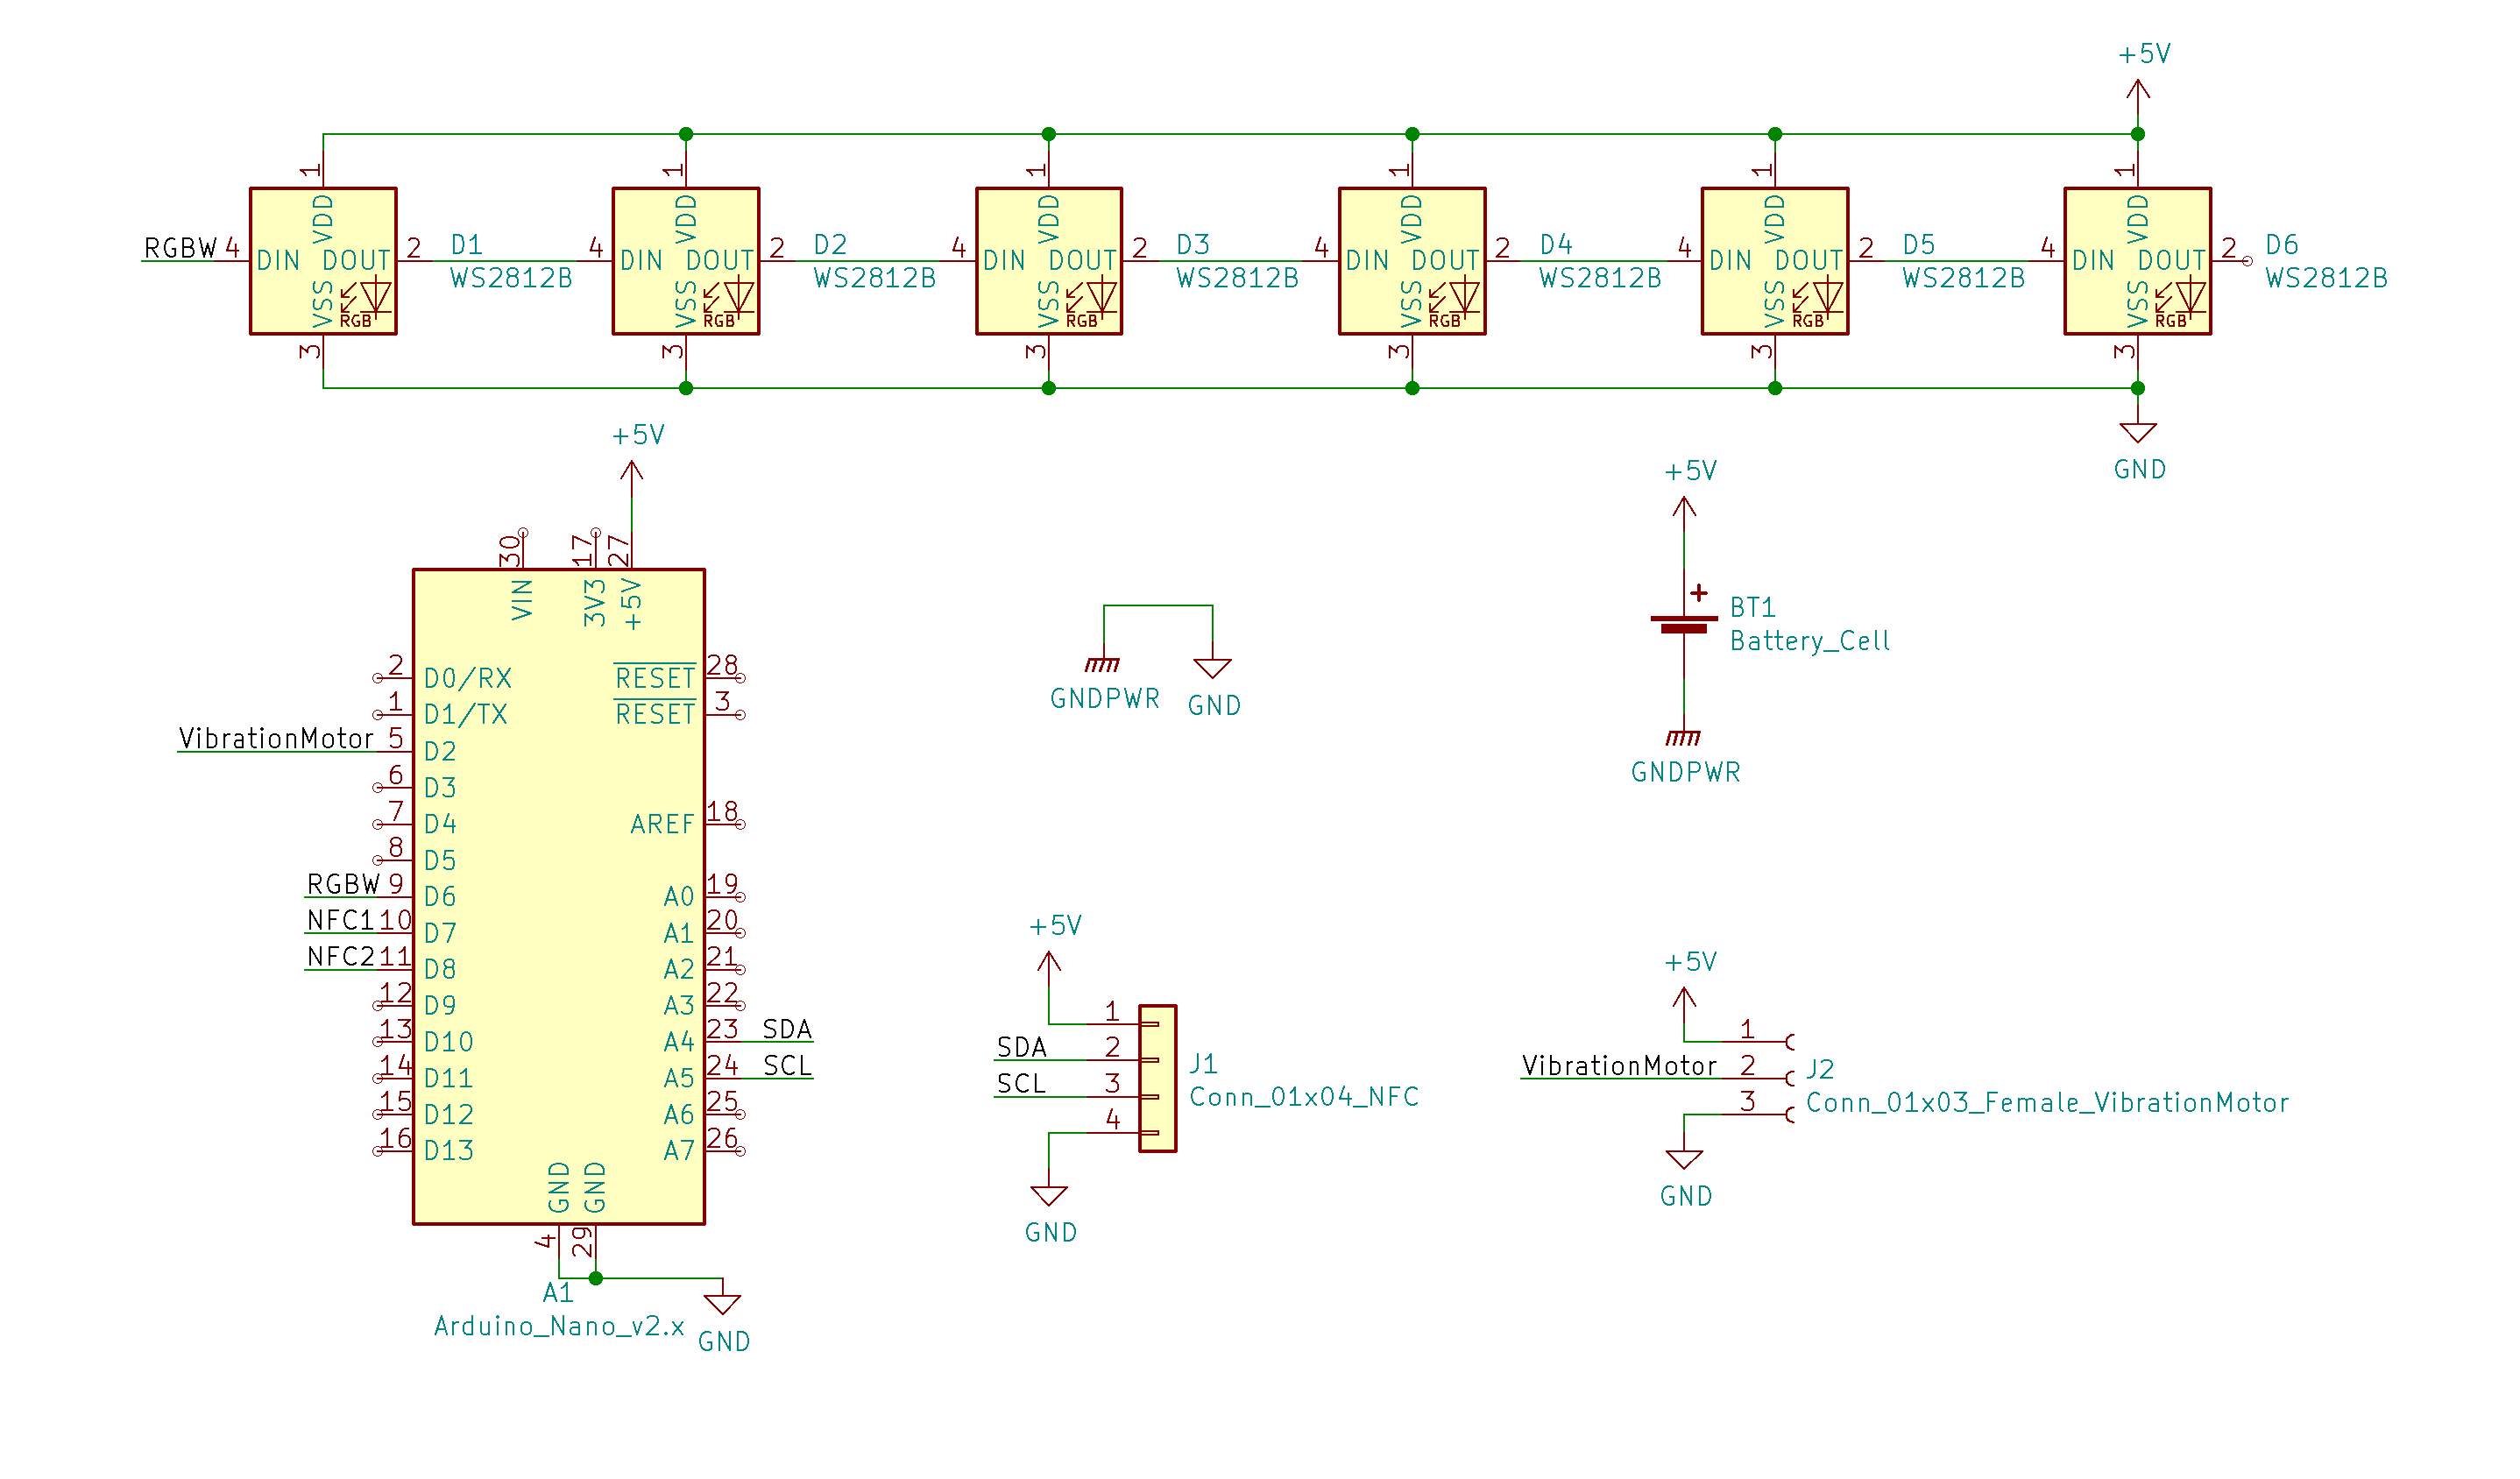
\includegraphics[width=\linewidth]{PCBsch1.png}
  \caption{The main PCB schematic}
  \label{PCBsch1}
\end{figure}

\begin{figure}
  \begin{minipage}{0.49\columnwidth}
    \centering
    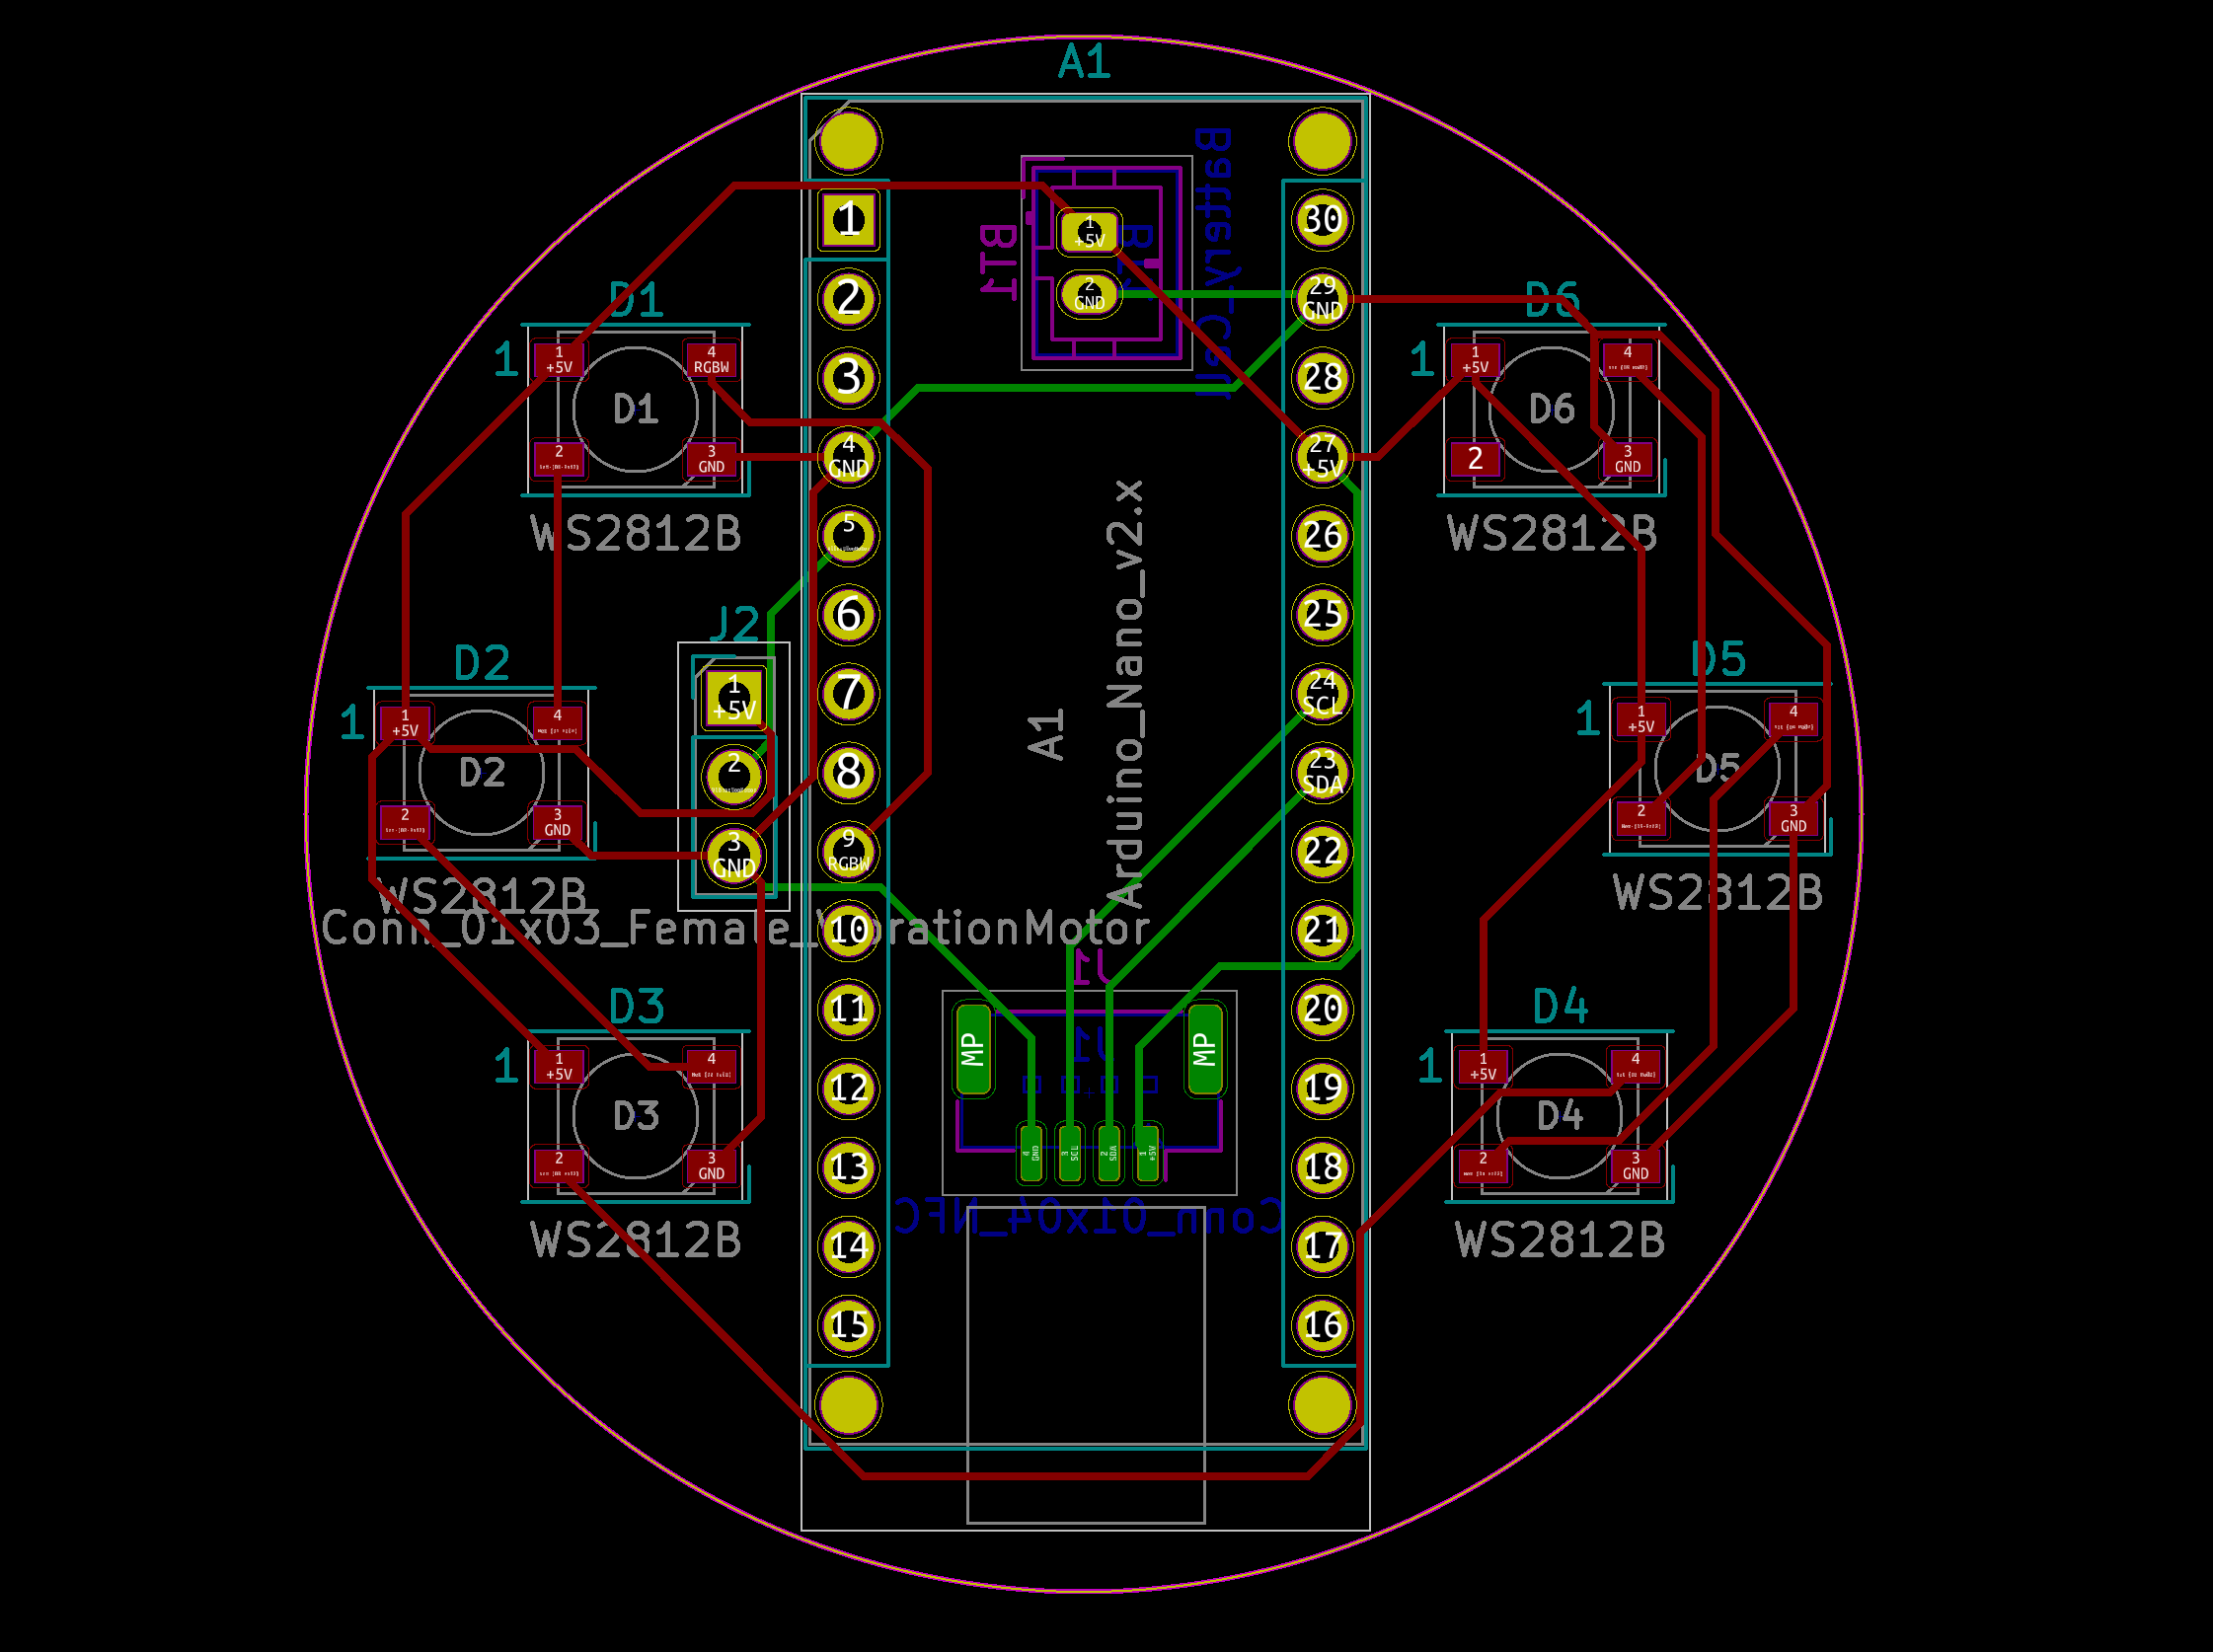
\includegraphics[width=0.99\columnwidth]{PCB1.png}
    \caption{The main PCB layout}
    \label{PCB1}
  \end{minipage}\hfill
  \begin{minipage}{0.49\columnwidth}
    \centering
    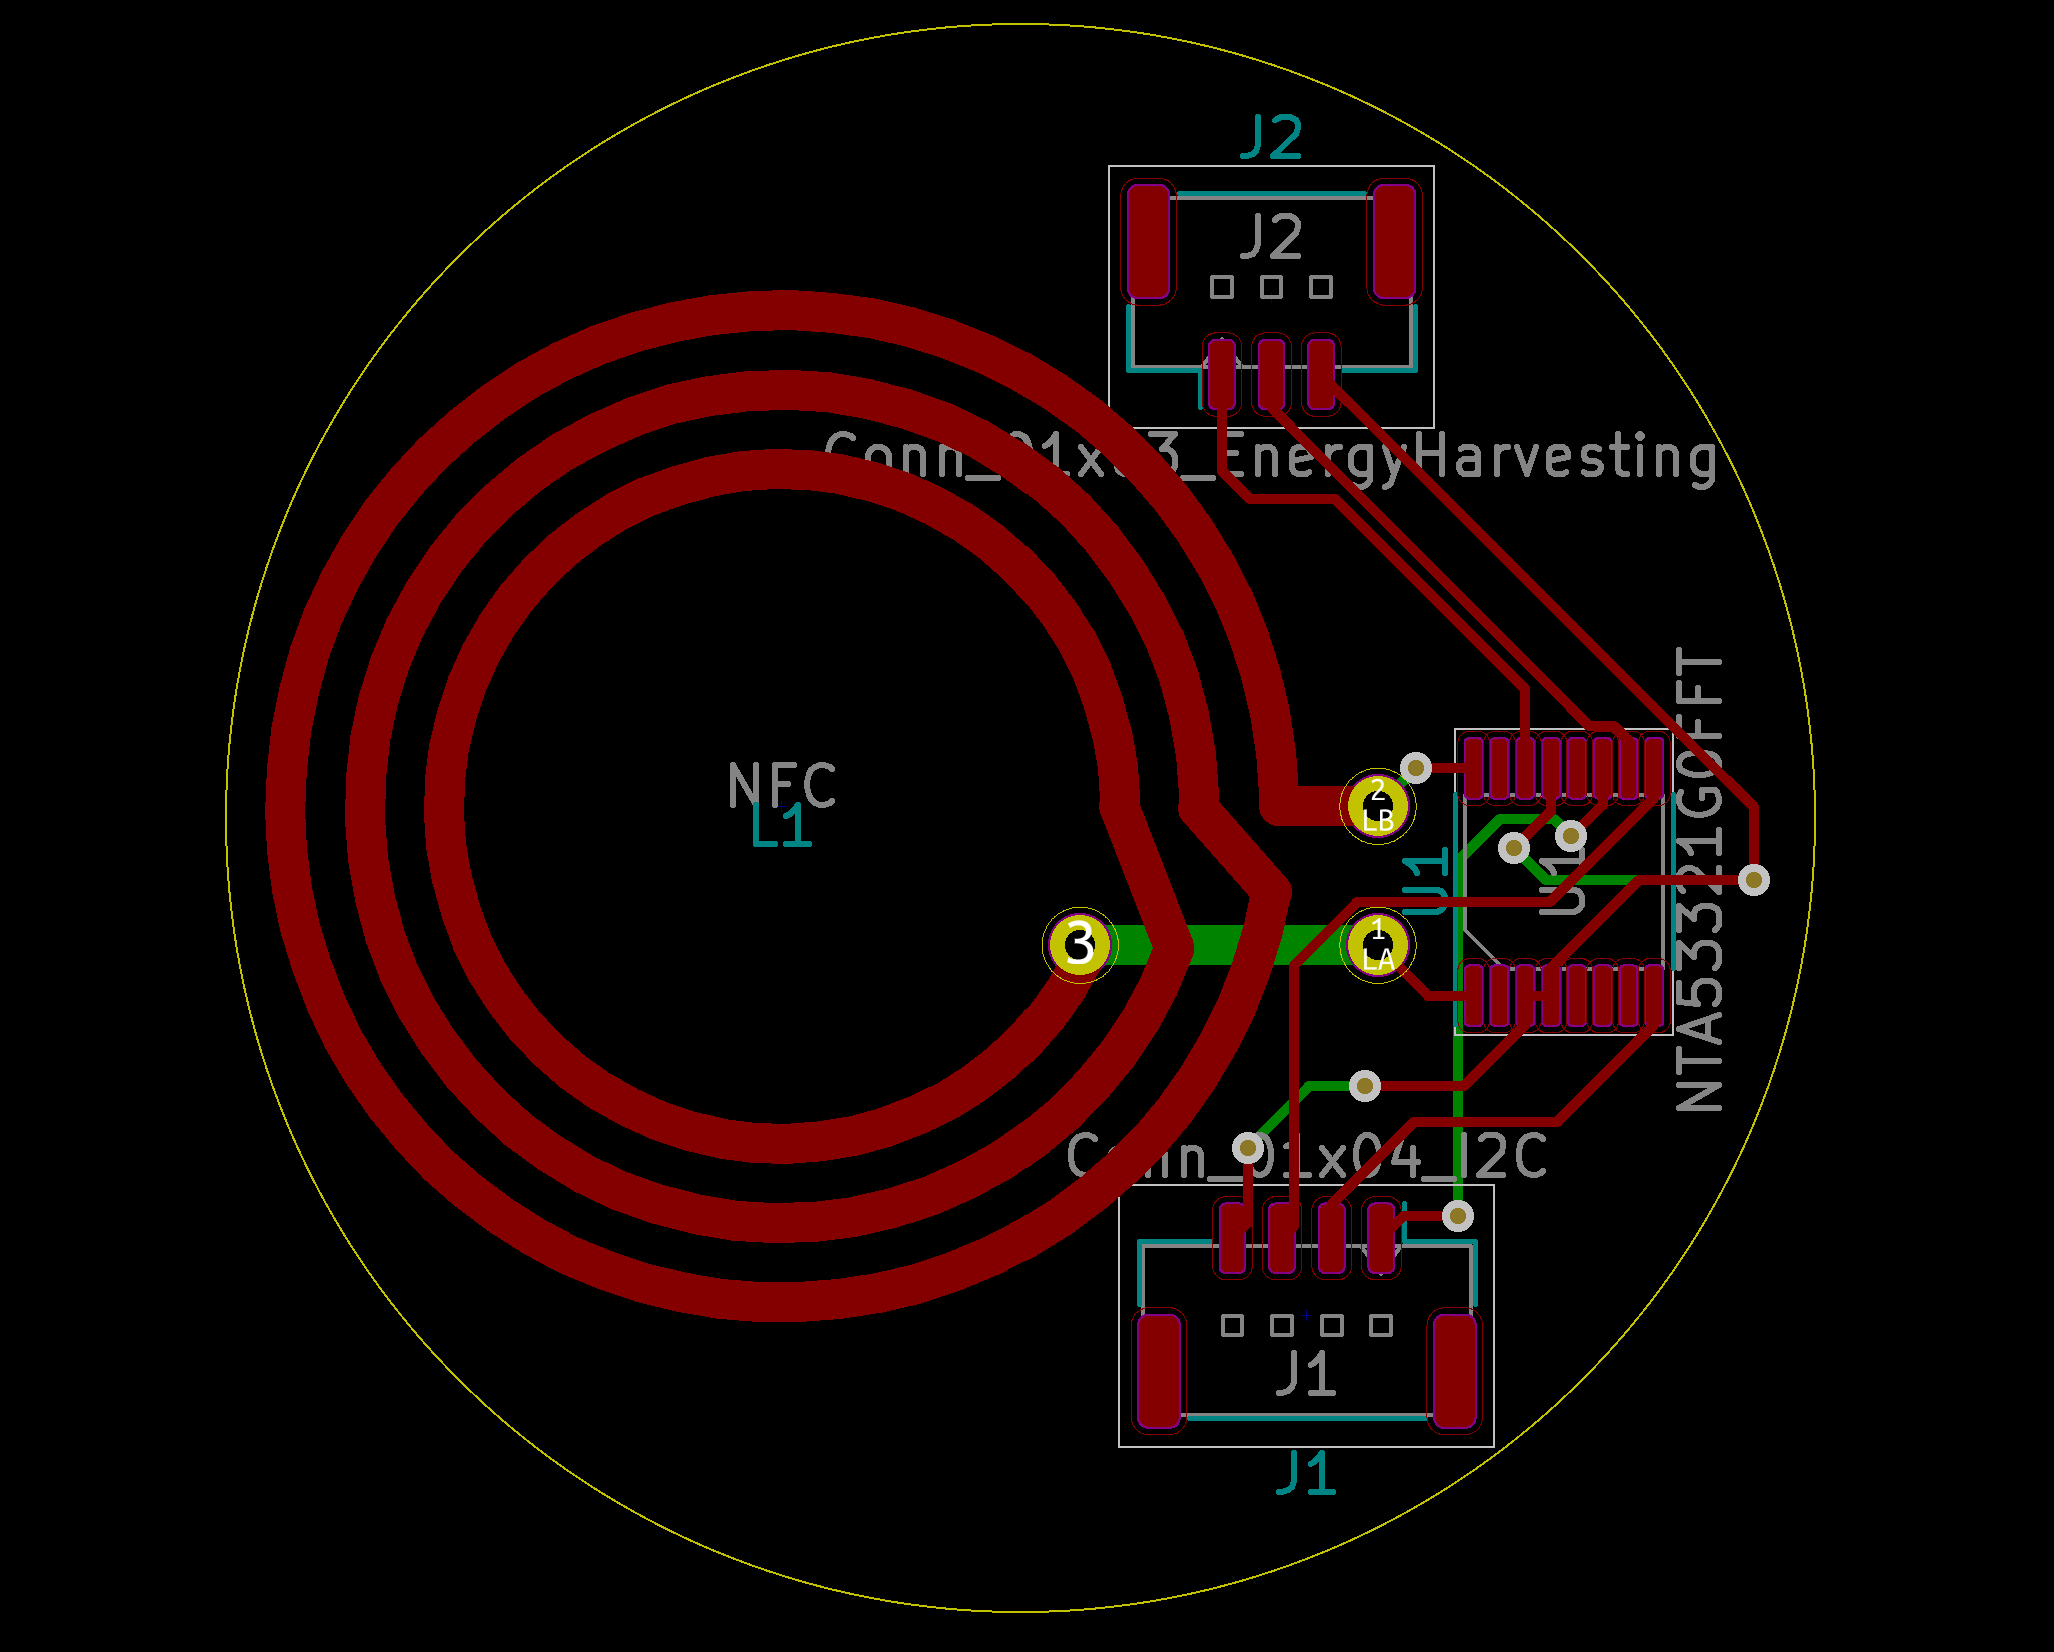
\includegraphics[width=0.99\columnwidth]{PCB2.png}
    \caption{NFC-PCB layout}
    \label{PCB2}
  \end{minipage}
\end{figure}

Also, Arduino Nano 33 BLE Sense supports NFC, we cannot drain power from the NFC coil using Arduino itself. It's necessary to add a chip to support wireless charging. We decide to use NXP and embedded it on the coil PCB. The communication protocol between NXP and Arduino is I2C.

SUSI Gene is illuminated in RGBW using WS2812B on the main PCB which are wrapped inside the 3D printed enclosure to provide the robot’s state display as well as full color indicating. As shown in Fig~\ref{Illum}.

\begin{figure}[h]
  \centering
  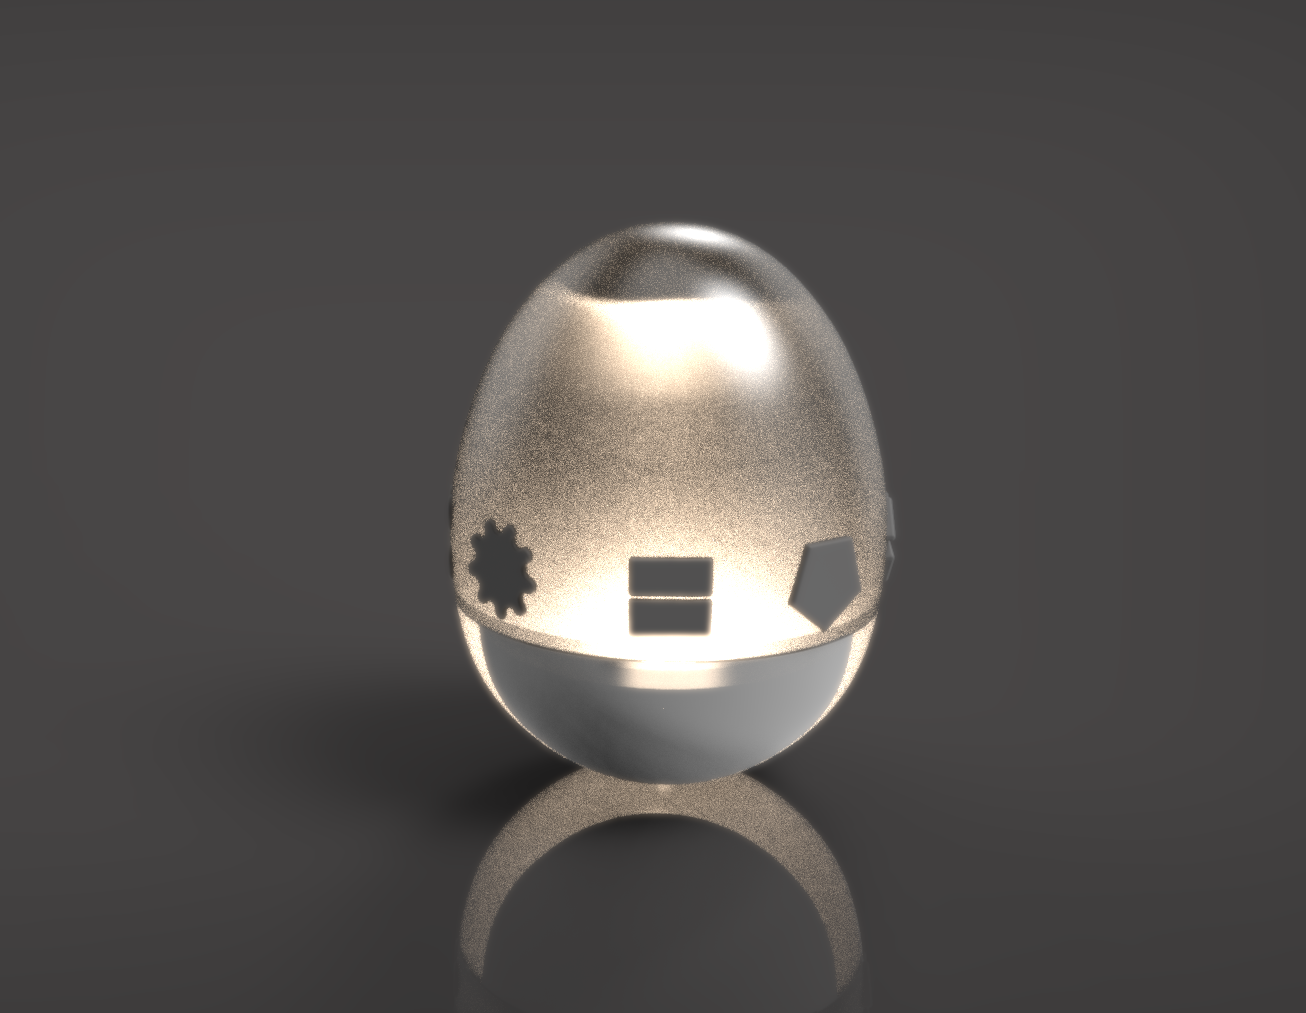
\includegraphics[width=0.7\linewidth]{egg4.jpg}
  \caption{Illuminated SUSI GENE}
  \label{Illum}
\end{figure}

The communications chipset on the Nano 33 BLE Sense can be both a BLE and Bluetooth client and host device. The main communication method between SUSI GENE and your phone is BLE.

The IMU(LSM9DS1) can detect the movement of SUSI GENE. When the user moves or touches the egg, it will vibrate or glomming depending on current feelings.

\subsection{Power consumption analysis}

SUSI Gene is powered by a 4000mAh 5V battery(3.7V 1S LiPo with boost PCM). Most of the power in the robots are consumed by the LEDs and Arduino. The current draw is approximately 200 mA during typical use. Thus, with a 4000 mAh battery, SUSI Gene is capable of working for about 20 hours without NFC wireless charging. Furthermore, with the ultra-low power consumption modes of Arduino, it can work longer when enabled.

\subsection{NLP solution}

One of the most important reasons for using Arduino Nano 33 BLE Sense is that it has the ability of Embedded Artificial Intelligence. It is possible to run Edge Computing applications (AI) on Nano 33 BLE Sense using TinyML. We can create our machine learning models using TensorFlow Lite and upload them to it using the Arduino IDE. The microphone(MP34DT05) can record your voice information. With those features, we can get voice recognition results with the NLP model.

However, the calculating ability of Arduino is too low to run complex algorithms. After lots of effort, it can only recognize simple phrases. At last, we decide to use a smartphone and its microphone instead. But soon, we will integrate the NLP process in SUSI GENE itself by using a more powerful chip supporting TensorFlow or other machine learning algorithms. 

\subsection{NFC PCB}

With an NFC tag at the bottom of SUSI GENE, the smartphone can recognize it using different UID of NFC tags and begin timing.

If users' smartphones do not have NFC, we provide an egg nest using NXP CLRC663 plus (High-performance NFC frontends) and connecting with the smartphone by BLE.

We use NXP NTA53321G0FTT(NTAG 5 boost: NFC Forum-compliant I2C bridge for tiny devices) as re-programmable NFC forum type 5 tag. It can harvest up to 30 mW energy when used as passive regulated.

NTAG 5 boost should be used for antennas smaller or equal class 6. For larger antennas, NTAG 5 link or switch should be used. So in this case, we use the NXP NFC Antenna Design Tool to design a class 6 antenna for NTAG 5 boost. The antenna of a “Class 6” design shall be located within a zone defined by a circle of 25mm diameter.

The NFC PCB schematic is shown in Fig~\ref{PCBsch2} and its layout is shown in Fig~\ref{PCB2}.

\begin{figure}[h]
  \centering
  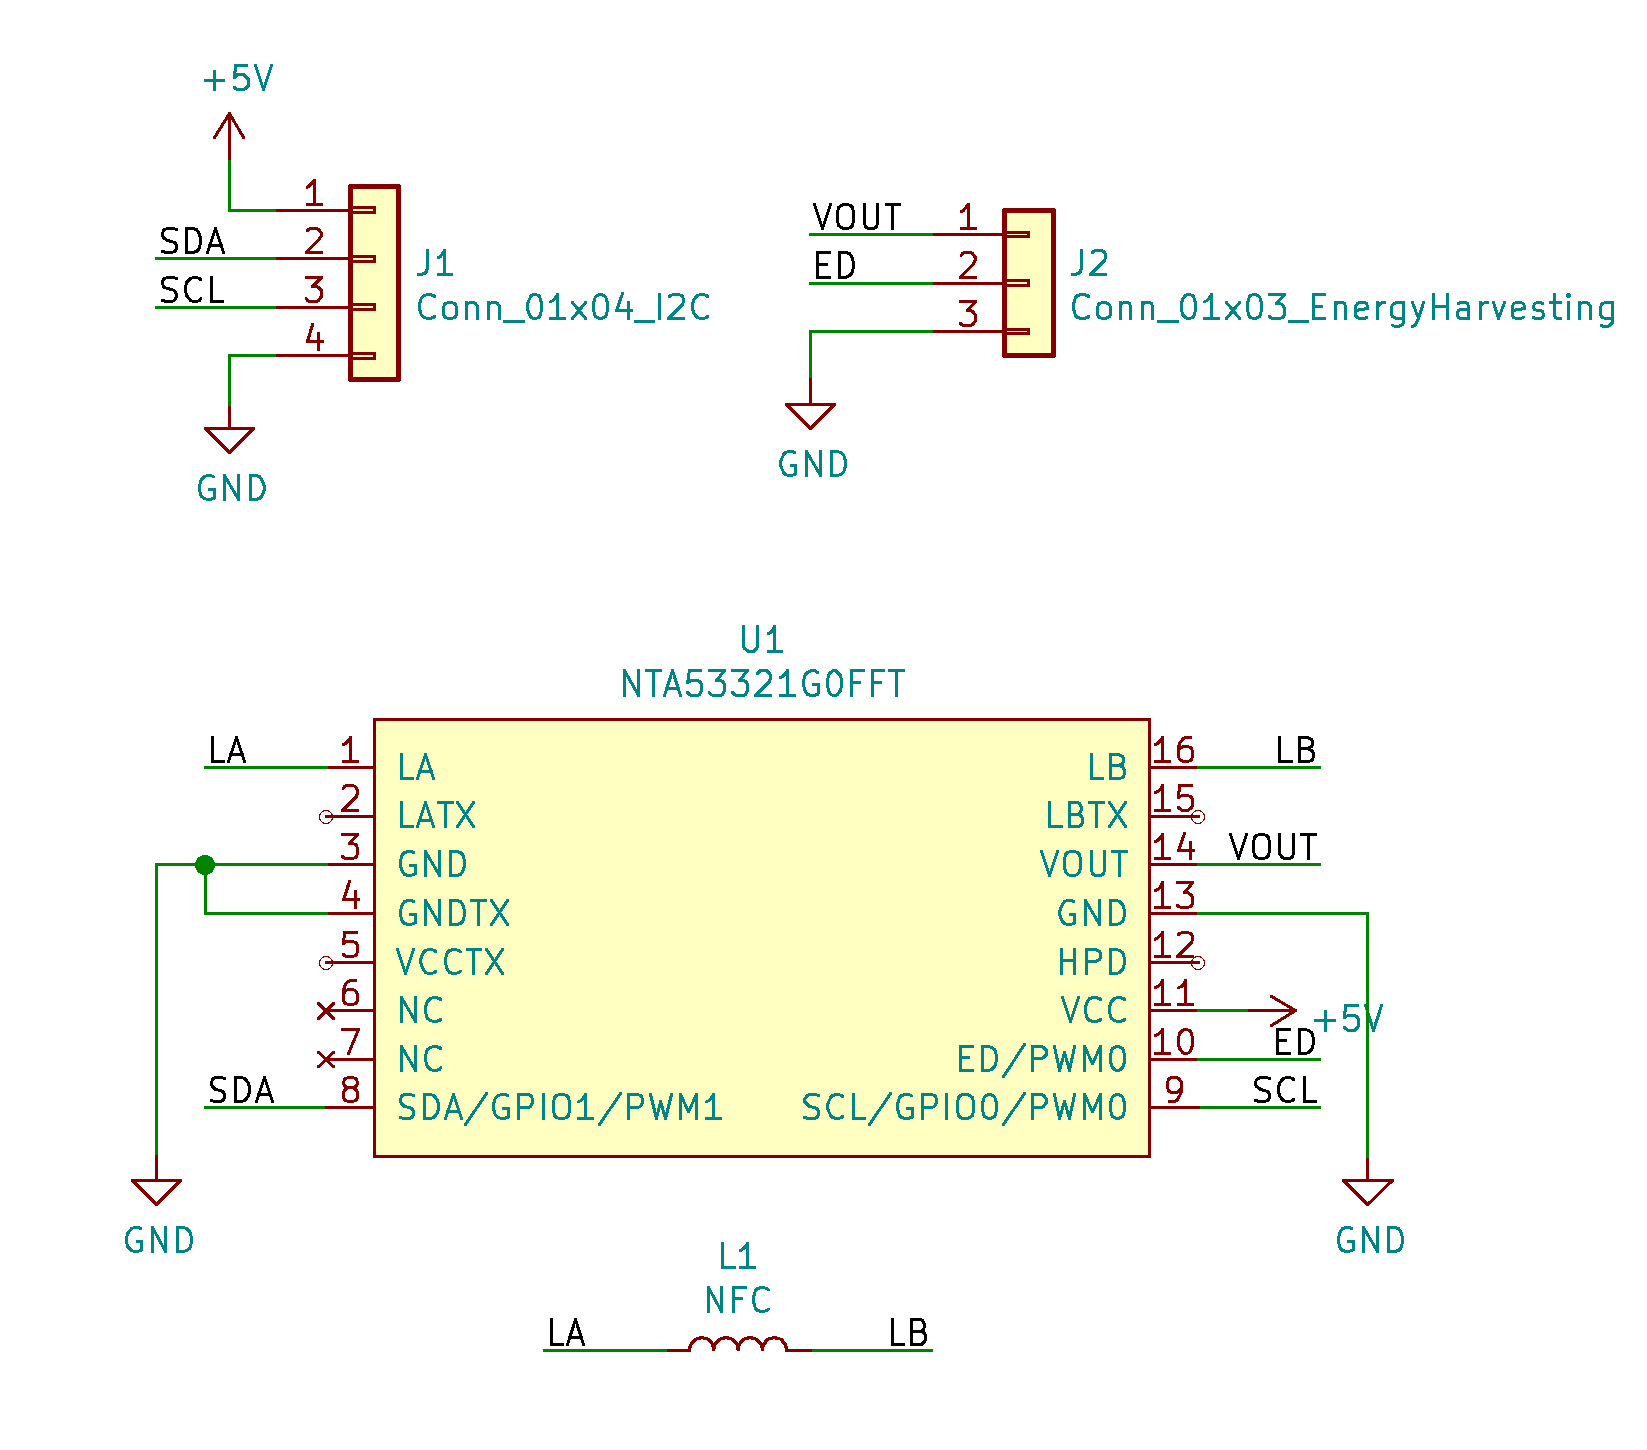
\includegraphics[width=0.7\linewidth]{PCBsch2.png}
  \caption{NFC-PCB schematic}
  \label{PCBsch2}
\end{figure}

\section{Discussion and future work}

In the future, we wish to integrate the NLP process in SUSI GENE itself by using a more powerful chip supporting TensorFlow or other machine learning algorithms. 

If we still want to put NLP on a smartphone instead of an embedded system, we can also use nRF52840 rather than Arduino Nano 33 BLE Sense to make the egg smaller and more efficient.

With much more powerful chips, we can make SUSI GENE smaller, more efficient, and more portable. 

We will find some people who suffer from mood disorders and do some user experiences and field surveys. Due to the COVID-19 pandemic, we have difficulty in UEX. But one of us suffers from bipolar disorder, and she comes up with this idea. Another member has a major depressive disorder, he tries most functionality of SUSI GENE, and give mostly positive feedback.

%%
%% The next two lines define the bibliography style to be used, and
%% the bibliography file.
\bibliographystyle{ACM-Reference-Format}
\bibliography{SUSI}

\end{document}
\endinput
%%
%% End of file `sample-manuscript.tex'.
